\documentclass[border=2pt]{standalone}
\usepackage{tikz}
\usetikzlibrary{arrows.meta,positioning}
\begin{document}
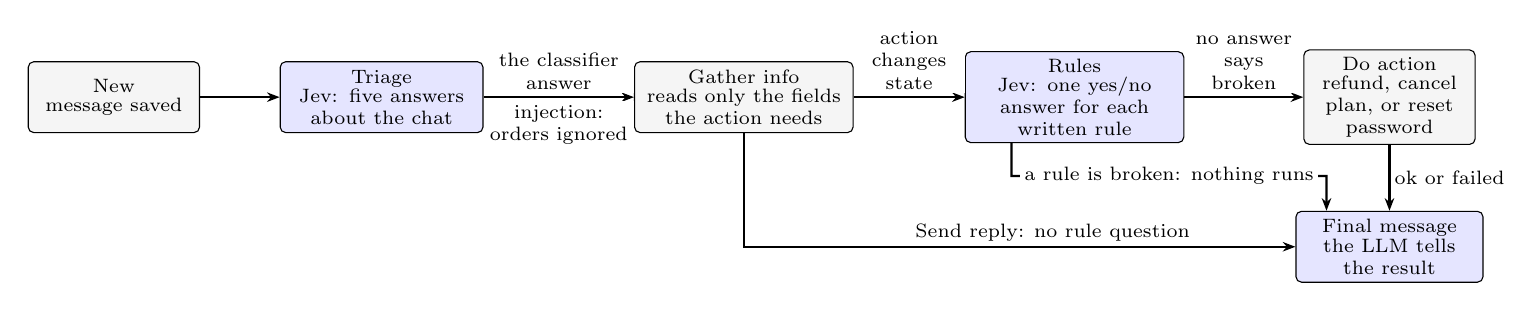
\begin{tikzpicture}[
  every node/.style={font=\scriptsize},
  st/.style={draw, rounded corners=2pt, minimum height=9mm, text width=20mm, align=center, inner sep=2.5pt},
  fx/.style={st, fill=gray!8},
  md/.style={st, fill=blue!10},
  rl/.style={st, fill=green!14},
  ar/.style={-{Stealth[length=1.6mm]}, thick},
  lb/.style={font=\scriptsize, inner sep=1.5pt, fill=white, text width=16mm, align=center},
  lw/.style={font=\scriptsize, inner sep=1.5pt, fill=white}]
  \node[fx] (new) at (0,0) {New\\[-1pt]{\scriptsize message saved}};
  \node[md, text width=24mm] (tri) at (3.4,0) {Triage\\[-1pt]{\scriptsize Jev: five answers about the chat}};
  \node[fx, text width=26mm] (gat) at (8.0,0) {Gather info\\[-1pt]{\scriptsize reads only the fields\\the action needs}};
  \node[md, text width=26mm] (rul) at (12.2,0) {Rules\\[-1pt]{\scriptsize Jev: one yes/no answer for each written rule}};
  \node[fx] (act) at (16.2,0) {Do action\\[-1pt]{\scriptsize refund, cancel plan, or reset password}};
  \node[md, text width=22mm] (fin) at (16.2,-1.9) {Final message\\[-1pt]{\scriptsize the LLM tells the result}};

  \draw[ar] (new) -- (tri);
  \draw[ar] (tri) -- node[lb, above=1pt, text width=18mm]{the classifier answer} node[lb, below=1pt, text width=18mm]{injection: orders ignored} (gat);
  \draw[ar] (gat) -- node[lb, above=1pt, text width=13mm]{action changes state} (rul);
  \draw[ar] (gat.south) |- node[lw, above, pos=0.78]{Send reply: no rule question} (fin.west);
  \draw[ar] (rul) -- node[lb, above=1pt, text width=13mm]{no answer says broken} (act);
  \draw[ar] (act) -- node[lw, right]{ok or failed} (fin);
  \draw[ar] ([xshift=-8mm]rul.south) -- (11.4,-1.0) -- (15.4,-1.0) -- ([xshift=-8mm]fin.north);
  \node[lw] at (13.4,-1.0) {a rule is broken: nothing runs};
\end{tikzpicture}
\end{document}
